\begin{figure}[h]
	\centering
	\missingfigure{Komponentendiagramm}		
	\caption{Komponentendiagramm - A}
	\label{fig:komponentendiagramm-a}
\end{figure}

\begin{tcolorbox}
Die strukturelle Übersicht des zu entwickelnden Systems wird mittels Komponentendiagrammen modelliert. 
Auf jedes Diagramm muss eine textuelle Beschreibung (Fließtext mit Umbrüchen / Absätzen oder Tabelle) folgen, in der die Aufgaben der Subkomponenten beschrieben werden. 
\end{tcolorbox}
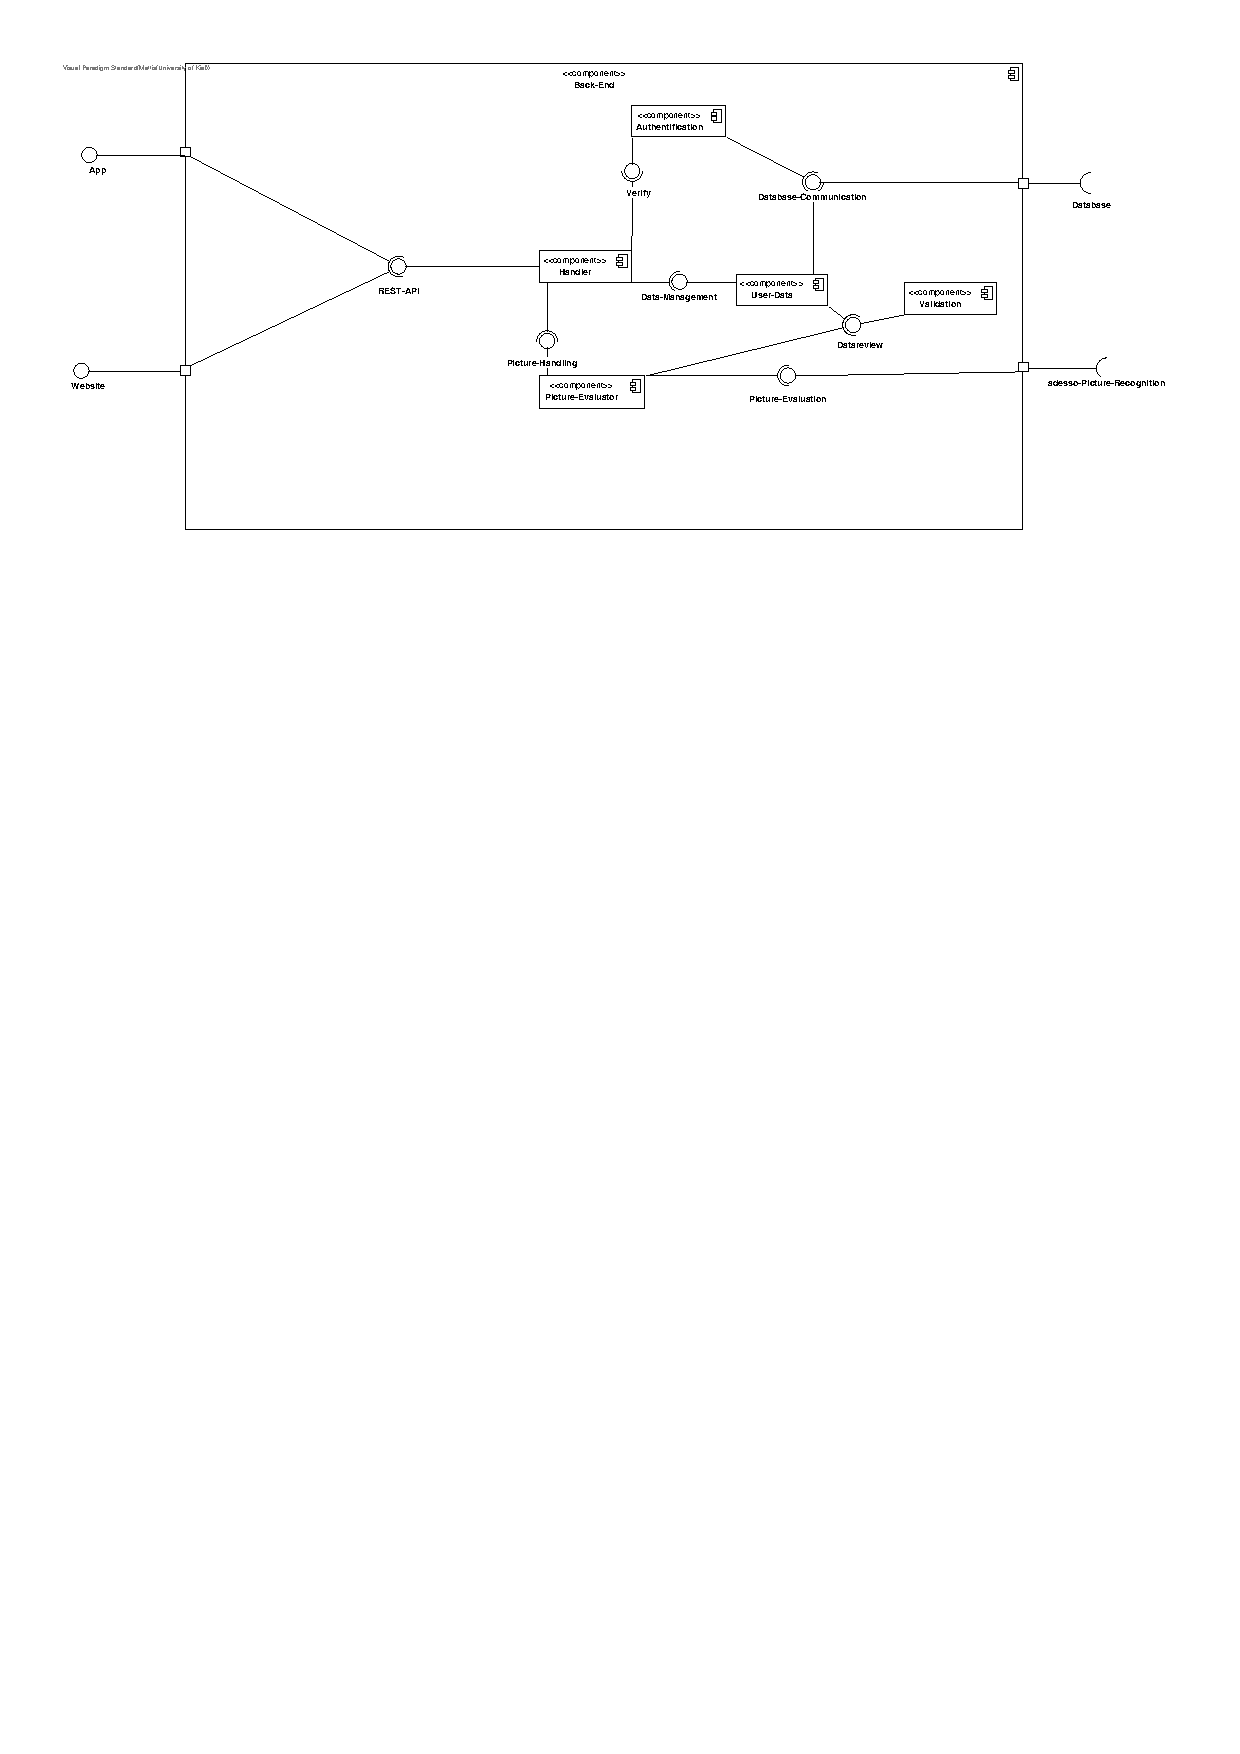
\includegraphics[scale=0.3]{\img\Komponenten_Back-Log}
Zusammengesetzt ist das ''Back-End'' aus mehreren Komponenten und Schnittstellen, die untereinander interagieren.\\
Dabei regelt die ''Handler''-Komponente den Dateneingang durch Nutzeranfragen, indem sie die Daten an die für sie zuständigen Subkomponenten weiterleitet. Dies geschieht über die von diesen Komponenten angebotenen Schnittstellen. Die Nutzeranfragen aus App und Browser werden dabei durch die ''REST-API''-Schnittstelle angenommen, welche von der ''Handler''-Komponente zur Verfügung gestellt wird.\\
Um zu überprüfen ob Nutzer privilegiert sind bestimmte Anfragen zu stellen existiert die ''Authentification''-Komponente. Diese verhindert damit, dass Nutzer Operationen durchführen, zu welchen sie nicht befugt sind. Zu diesem Zweck stellt sie dem ''Handler'' eine ''Verify''-Schnittstelle zur Verfügung. Um die Befugnis eines Benutzers für eine bestimmte Operation zu überprüfen, benutzt die ''Authentifikation'' die ''Database-Communication''-Schnittstelle. Über diese werden die benötigten Rechte mit den in der Datenbank gespeicherten Rechten des Benutzers abgeglichen.\\
Weiterhin wird diese ''Data-Communication''-Schnittstelle von der ''User-Data''-Komponente genutzt. ''User-Data'' ermöglicht bei entsprechenden Privilegien das Abrufen oder Ändern von Kundendaten. Diese Komponente wird insbesondere genutzt um Zählerstände zu aktualisieren.\\
Die gewünschten Zugriffe auf Kundendaten erfolgen über die von der ''User-Data''-Komponente bereitgestellte ''Data-Management''-Schnittstelle, welche von der ''Handler''-Komponente verwendet wird.\\
Bei Veränderungen der Daten in ''User-Data'' werden diese durch die ''Datareview''-Schnittstelle an die ''Validation''-Komponente weitergeleitet. Dort werden Zählerstände und Nummern auf ihr Format, sowie Passwörter auf Sicherheitsstandards überprüft.\\
Auf die ''Data-Review''-Schnittstelle greift ebenfalls die ''Picture-Evaluator''-Komponente zu, um Zählernummern und Zählerstände auf Validität zu überprüfen. Diese Werte erhält die Komponenente von der ''adesso-Picture-Recognition'', welche die Bilder extern auswertet. Verbunden sind diese dabei über die ''Picture-Evaluation''-Schnittstelle. Die Bilder welche ausgewertet werden sollen gelangen über die ''Picture-Handling''-Schnittstelle, welche von der ''Picture-Evaluator''-Komponente angeboten wird, in eben diese. Umgekehrt werden die daraus erhaltenen Daten über die gleiche Schnittstelle an die ''Handler''-Komponente zurückgesendet. Die ''Picture-Evaluator''-Komponente fungiert somit als Knotenpunkt für die Bildverarbeitung. 
